\documentclass{article}
\usepackage{../fasy-hw}

%% UPDATE these variables:
\renewcommand{\hwnum}{5}
\title{Discrete Structures, Homework \hwnum}
\author{Peyton Meeks}
\collab{n/a}
\date{due: 19 March 2021}

\begin{document}

\maketitle

This homework assignment should be
submitted as a single PDF file both to D2L and to Gradescope.

General homework expectations:
\begin{itemize}
    \item Homework should be typeset using LaTex.
    \item Answers should be in complete sentences and proofread.
    \item You will not plagiarize.
    \item List collaborators at the start of each question using the \texttt{collab} command.
    \item Put your answers where the \texttt{todo} command currently is (and
        remove the \texttt{todo}, but not the word \texttt{Answer}).
\end{itemize}


% ============================================
% ============================================
\collab{n/a} \nextprob{Colors}
% ============================================
% ============================================

One thing that we need to consider as computer scientists is making our products
(software, technical papers) accessible to a wide range of people. When
designing GUIs or writing technical papers (e.g., journal papers or even
homework solutions), explain five things that you could do to make your
technical write-ups, website, or GUI products more accessible to people who
might be colour deficient or have Colour deficiency(or have a bad computer screen).


\paragraph{Answer}
	\begin{enumerate}
		\item Using plain black text for journals and papers reduces chances of the reading being unaccesable to people. Also, using black text as much as possible gives a more formal and less distracing appearance to the text.
		\item By limiting the use of colors to images or special text/characters allows them to provide contrast to the document which will grab the readers attention and allow for the reader to assess what is important in the document. By using colors that are typically not associated with one another for color blindness, especially in figures or images with more than one color will allow audicences that suffer from color blindness to hopefully still understand the document.
		\item By using a appropriate font and font size for large clumps of block text will allow the audience to better read and digest the text without straining their eyes or their brains.
		\item By using descriptive captions on figures which thoroughly describe what is happining in the image also allow the audience to better understand the figure, even if seeing what is happening is not possible. This helps the reader build their own mental image of whats happening, thus helping if the reader cannot understand or see the provided image.
		\item Finally, by breaking up large blocks of text with a figure, if possible, or white space by breaking up one massive paragraph into multiple, creates a mental break in the readers subconcious causing the reader to pause even if it is for a very short time. This allows the reader to better digest what they have just read, while also making the overall flow of the text more controlled. By doing this it helps mental strain from staring at a huge chunck of words, especially if the readers using an older computer or has a small/bad computer screen.

	\end{enumerate}

% ============================================
% ============================================
\collab{n/a} \nextprob{The Complete Bipartite Graph $K_{n,n}$}
% ============================================
% ============================================

How many edges does the complete bipartite graph $K_{n,n}$ have?  Make your
conjecture, then prove that it is correct.

Bonus: Instead, prove the more general case:
what is the number of edges in $K_{n,m}$?

\paragraph{Answer}

Conjecture: A complete bipartite graph $K_{n,m}$ has $n*m$ edges. 

By definition of a complete bipartite graph, we know that a graph is a complete bipartite graph if its vertices can be divided into two distinct subsets $V_n$ and $V_m$. Therefore if $V$ is the set of all vertices in $K_{n,m}$ then$V_1 \subseteq V$ of size $n$ and $V_2 \subseteq V$ of size {m}. Then $V_n+V_m=V$ and $n+m=$ the total size of $V$. Then by definiton of a complete biparite graph, no edge can have both endpoints in the same subset and every possible edge that connects vertices in different subsets exists. So if $v_1$ is a vertex $\in V_n$ and $v_2$ is a vertex $\in V_m$ then the edge that connects those vertices would be $v_1v_2$. Since $n$ and $m$ are the size of the subsets $V_n$ and $V_m$ then $n*m$ would be the total number of edges for a complete biparite graph $K_{n,m}$.





% ============================================
% ============================================
\collab{Patrick OConner(322)} \nextprob{Four Colors Suffice}
% ============================================
% ============================================

Read Chapters $7$ and $8$ of \emph{Four Colors Suffice}.

\begin{enumerate}

    \item In the Four Colors Suffice book, we saw the definition of Euler's
        Formula for a finite decomposition of a Sphere or 2-plane into vertices,
        edges, and faces.  What is the other formula known as Euler's formula?

        \paragraph{Answer}

        Euler's Formula for a Torus: The number of Faces minus the number of Edges plus the number of Vertices equals 0, or $F-E+V=0$.



    \item  Consider the following construction: Start with a solid cube.  Then, slice
        off a small region around each vertex (image you have a sharp knife, so you take
        off a tetrahedron at each corner).  How many vertices, edges, and faces are on
        the surface of this object before and after this operation? What polyhedron is this?

        \paragraph{Answer}

        Before the sliceing of the regions, a solid cube consists of 8 vertices, 8 edges and 6 faces. After the slicing operation there are 24 vertices, 36 edges, and 14 faces. The slicing operation created a Truncated cube. \footnote{“List of Uniform Polyhedra.” Wikipedia, Wikimedia Foundation, 16 Mar. 2021, \url{en.wikipedia.org/wiki/List_of_uniform_polyhedra}.}


		\begin{figure}[h]
		\centering
			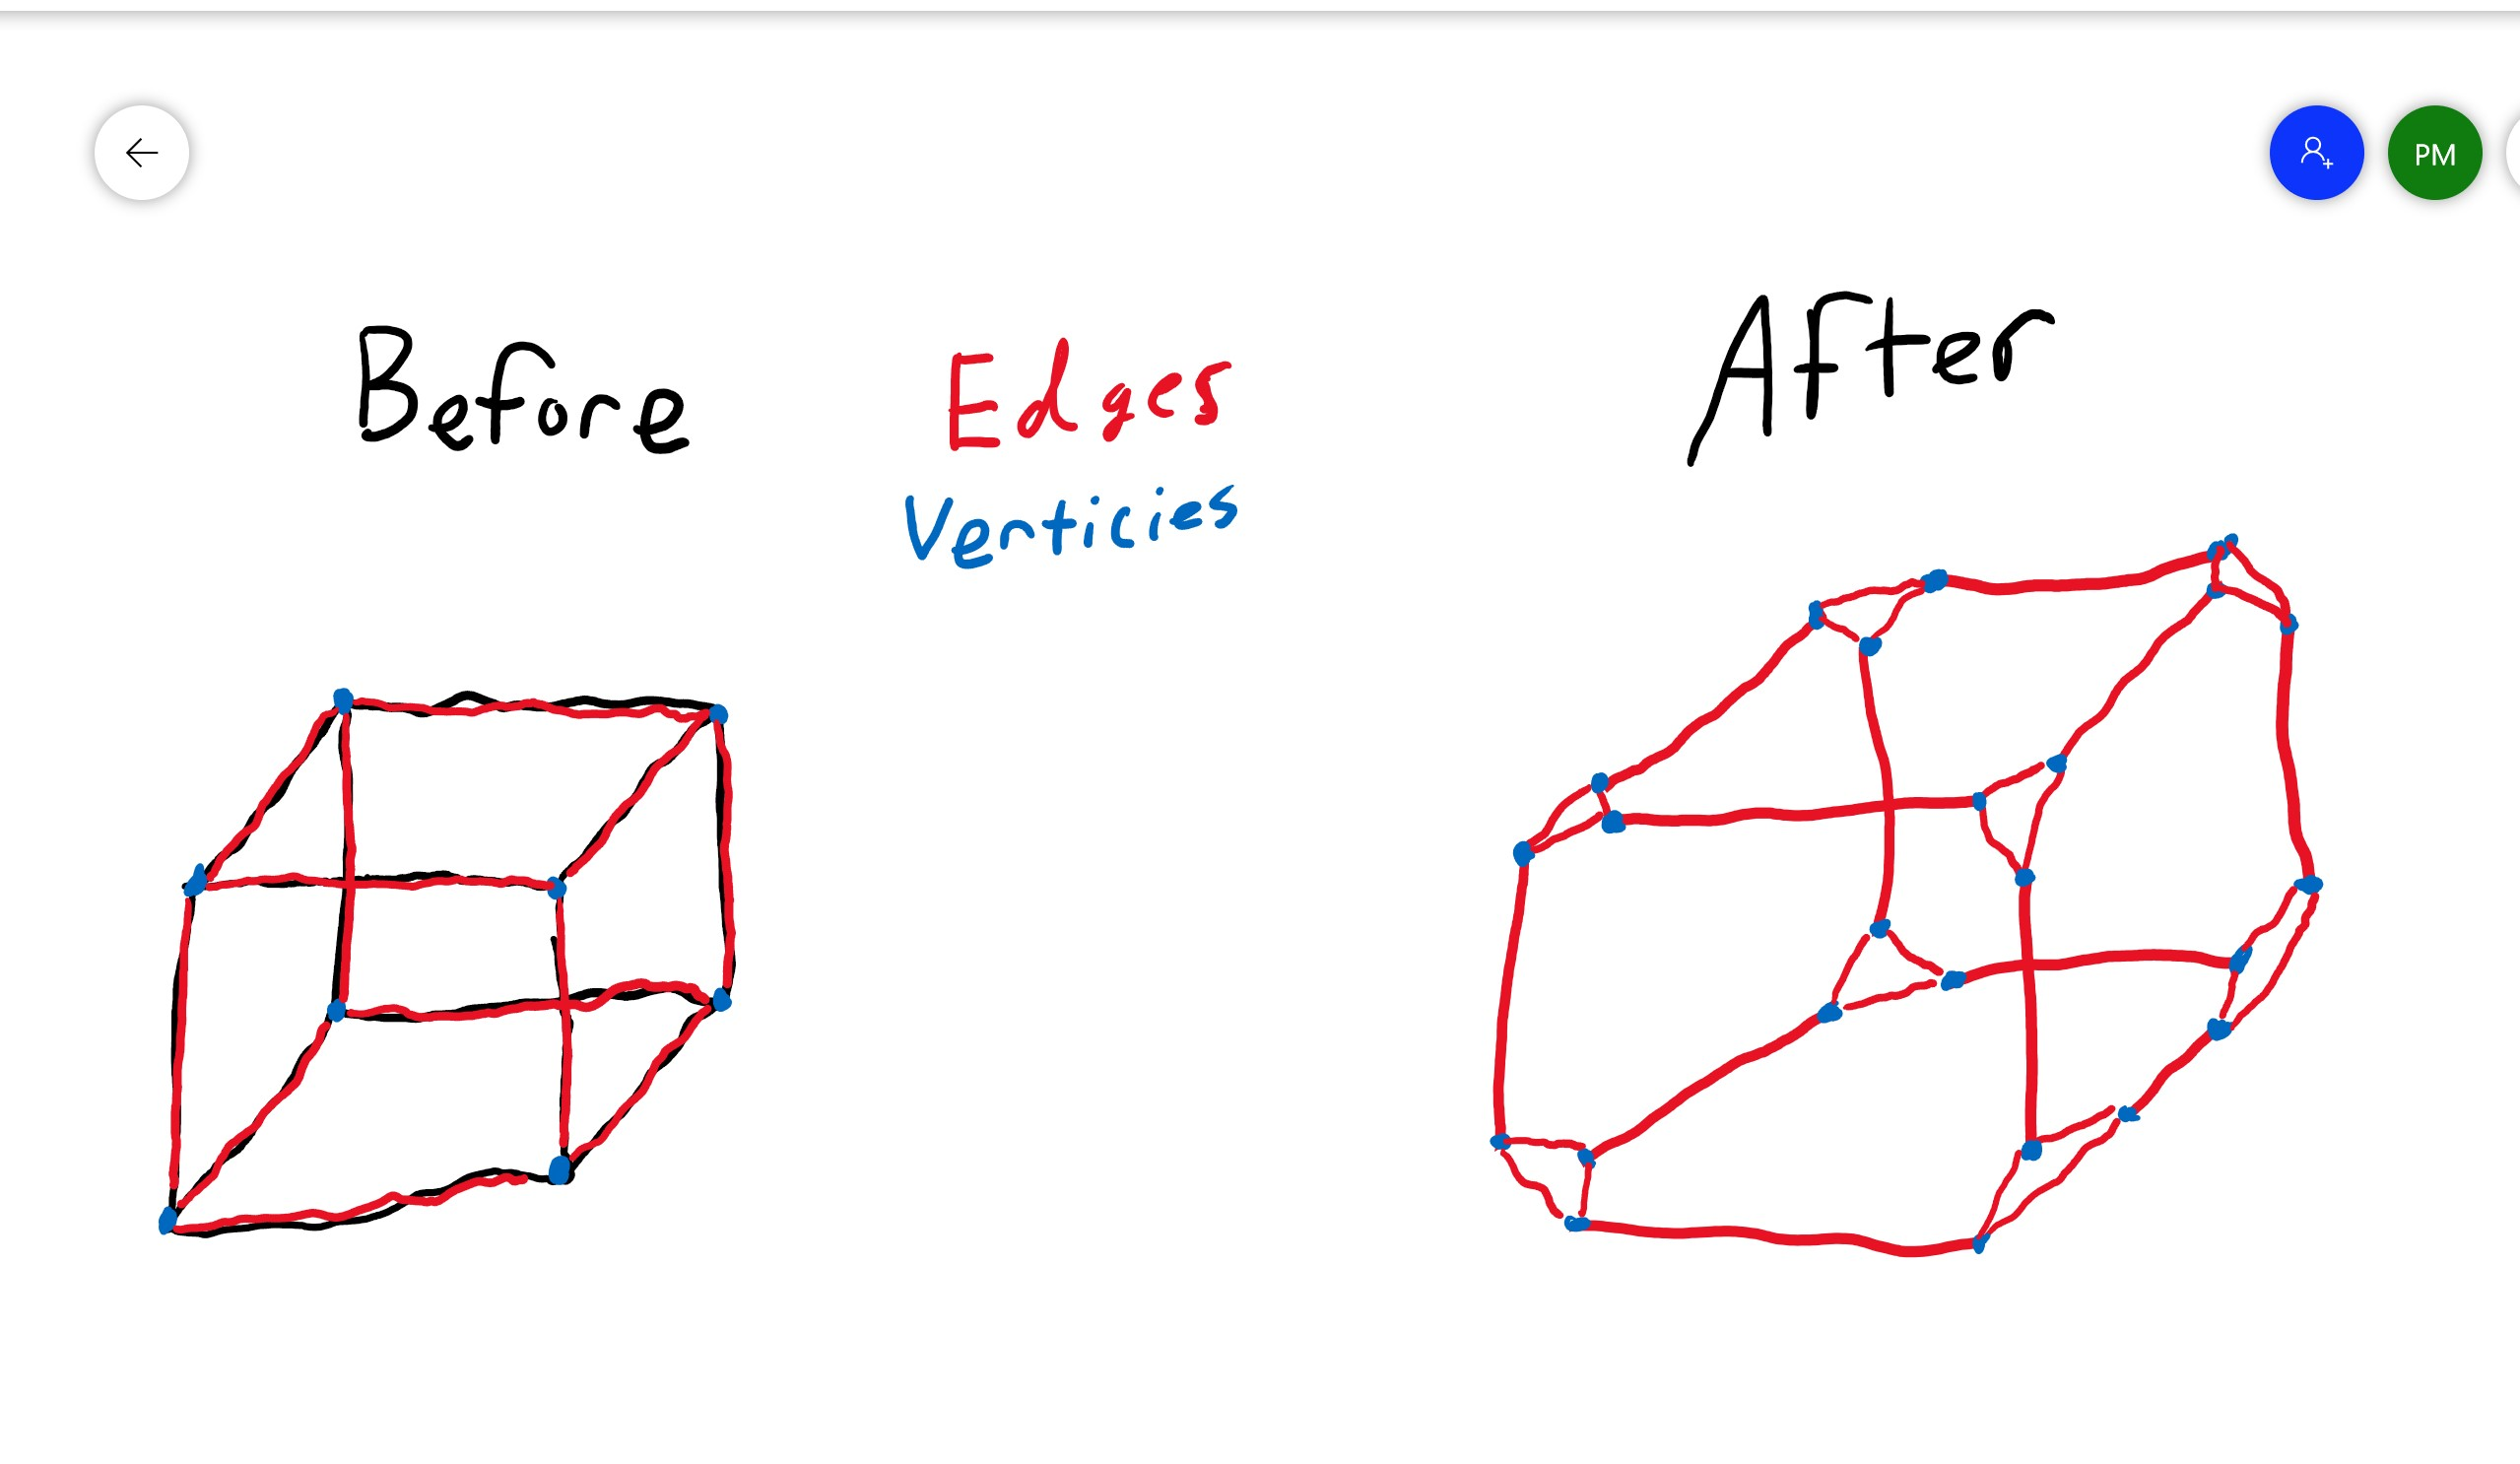
\includegraphics[width=0.25\textwidth]{HW_5_3-2}
		\end{figure}




    \item Draw a projection of the octahedron onto the plane such that edges only
        intersect at vertices.  Can every polyhedron be drawn in such a way?

        \paragraph{Answer}

		Yes, as long as the outside can be counted as a face, then all polyhedron can be drawn so that no edges intersect execpt for at vertices.

        \begin{figure}[h]
		\centering
			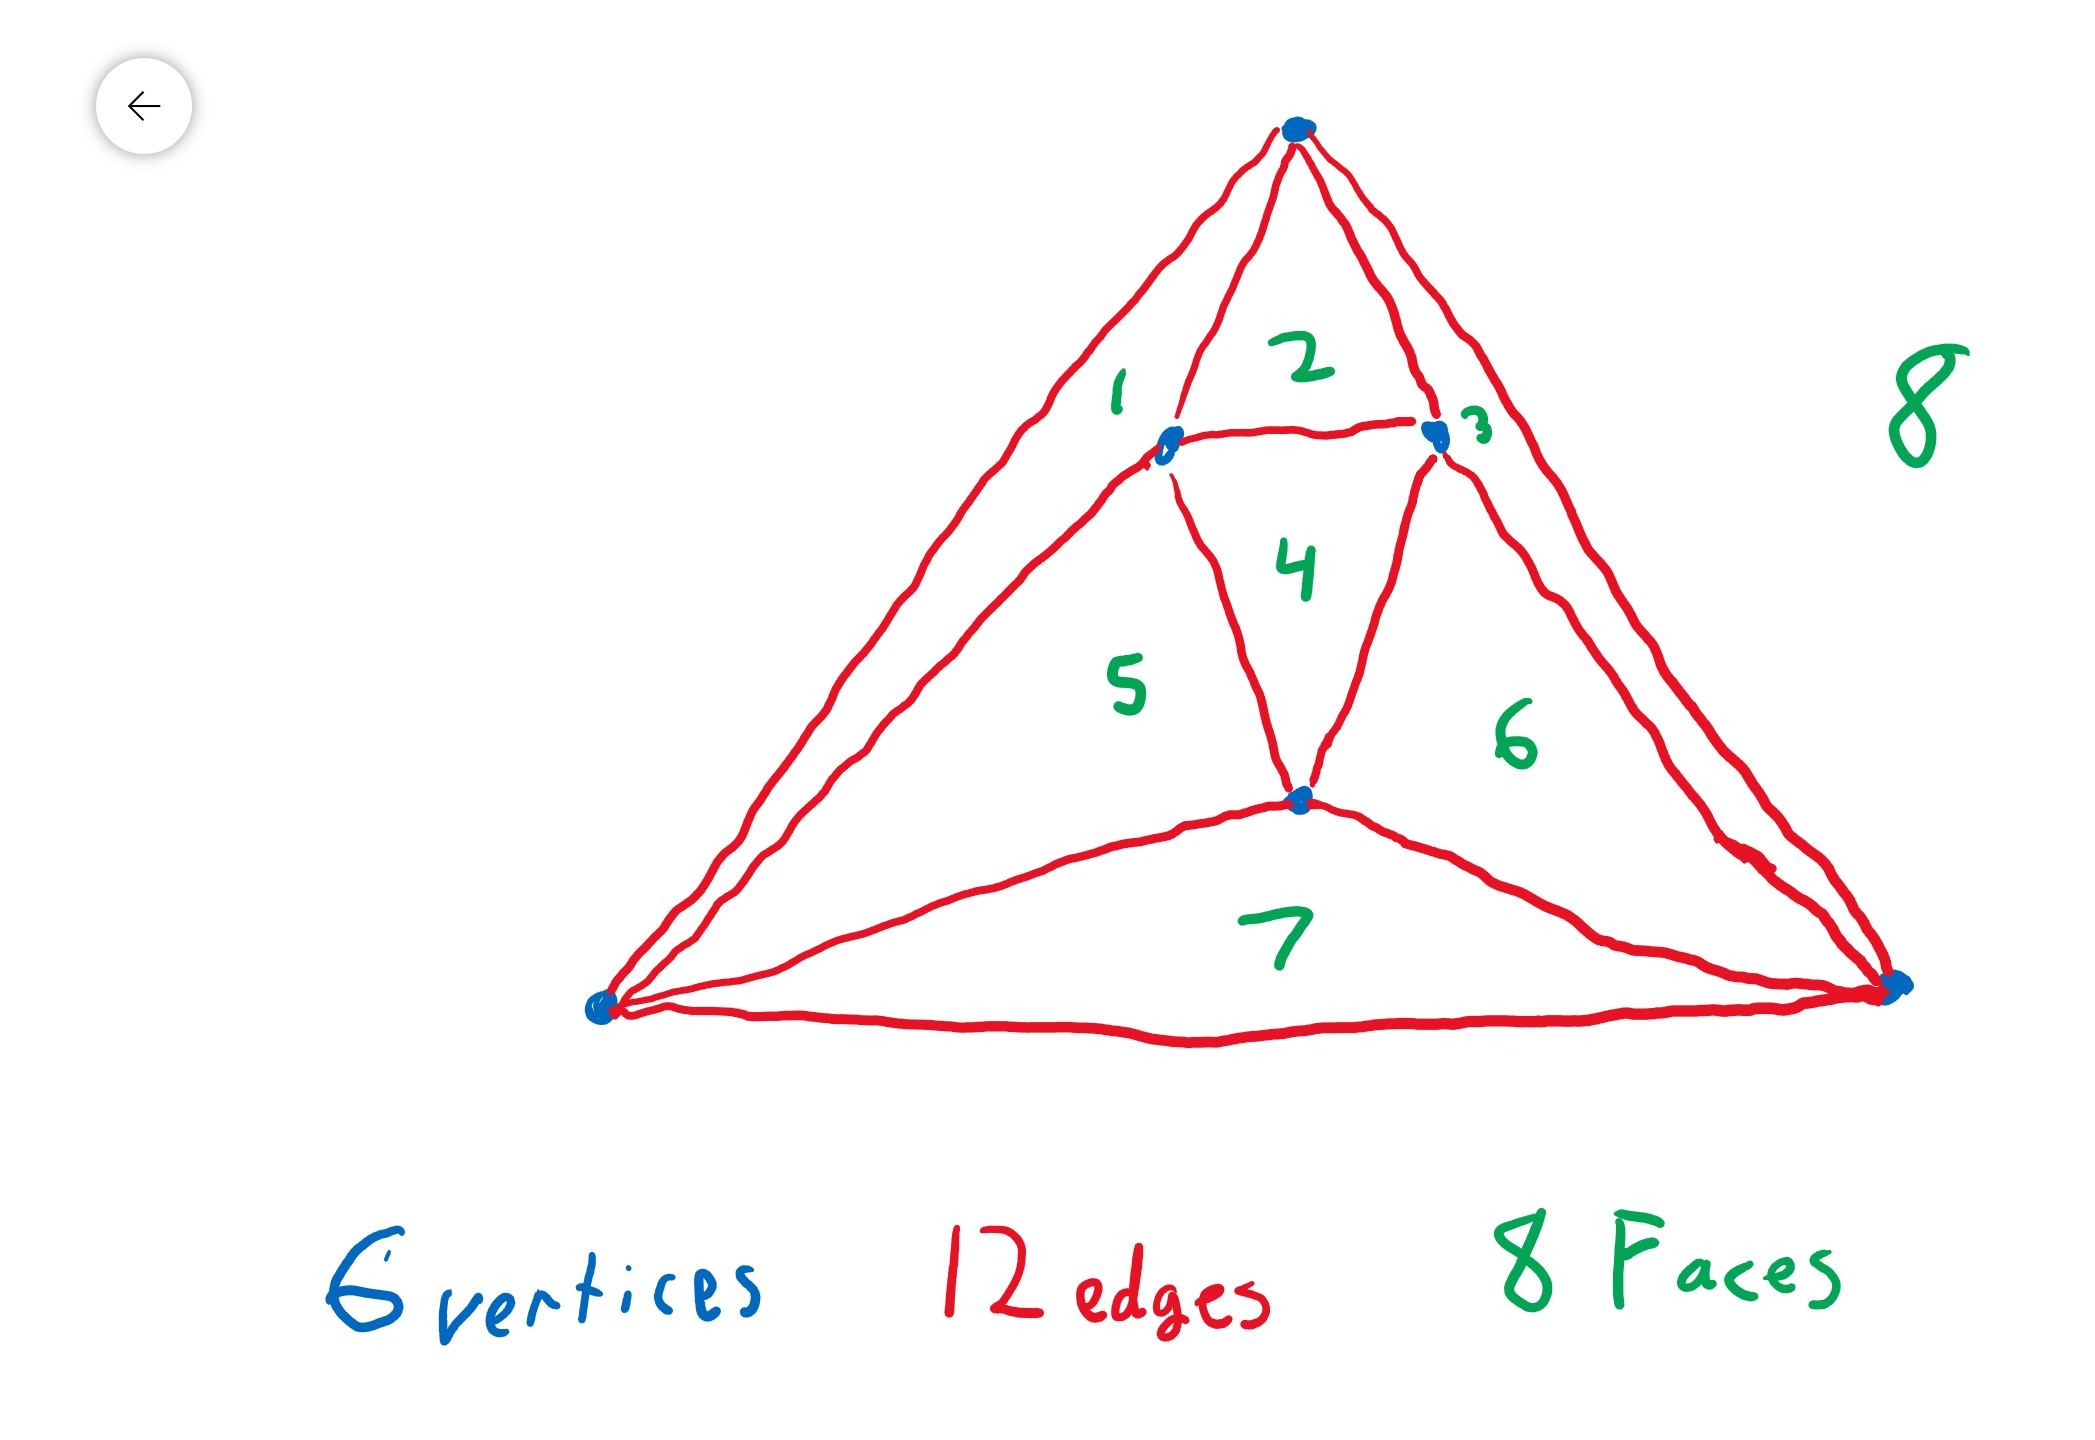
\includegraphics[width=0.25\textwidth]{HW_5_3-3}
		\end{figure}


\end{enumerate}

% ============================================
% ============================================
\collab{n/a}
\nextprob{Fran Allen}
% ============================================
% ============================================

Write a short (1-2 paragraph) biography of Fran Allen.
\textbf{In your own words}, describe who they are and why they are important in
the history of computer science.

If you use external resources, please provide
proper citations. If you do not use external sources, please write ``I did not
use any sources to write this biography'' as the last sentence of the
biography.

\paragraph{Answer}

Frances Allen was an American computer scientist who pioneered the world of computer science based on her research of compiling data. Allen was born August 4th, 1932 and grew up in Peru, New York.(I could not find an exact birthplace) She remained in New York through college, recieving her bachelor's degree in mathmatics from New York State College for Teachers. After college she was a teacher for a couple years back in her hometown before enrolling in college again at the University of Michigan. It was here that she recieved her master's degree and began her path to becoming one of the most prestigious researchers in computer science. 

After earning her master's degree Allen began working as a programmer for IBM Research back in New York. Allen worked on many projects in her 45 years of working for IBM. Some of these are helping develop a programming language, managing a compiler-optimization team for several projects with the NSA, and contributing to PL/I. It was at this time when she met John Cocke, another infamous computer scientist in the field of optimization. After this is when Allen made some of her greatest achivements, leading IBM's parallel computing project in the 1980's. This reasearch would lead to major advances in software development, allowing developers to create more compact and powerful code. This ripple effect allowed major advances in the efficiency of supercomputer's handling of upper level code. This is what earned Allen the title of ``The Pioneer of Compiling'' and eventually the Turing award, one of the highest awards in computer science. Frances Allen passed away on August 4th, her birthday, 2020 due to complications of Alzheimer's disease. Today she is still regarded as one of the most influencial members of computer development. Allen was also awarded a honorary doctorate of science for her contributions along with being a member of multiple engineering and science societies. \footnote{Spells, Alta. “Frances Allen, Pioneering Computer Scientist, Is Dead at the Age of 88.” CNN, Cable News Network, 9 Aug. 2020, \url{www.cnn.com/2020/08/09/us/frances-allen-death-obit/index.html}.} \footnote{“Frances Allen.” Wikipedia, Wikimedia Foundation, 17 Mar. 2021, .  \url{en.wikipedia.org/wiki/Frances_Allen}.}

% %% ... the bibliography
% \newpage
% \bibliographystyle{acm}
% \bibliography{biblio}

\end{document}

